\documentclass[a4paper,11pt]{jreport}

\usepackage[dvipdfmx]{graphicx}
\usepackage[dvipdfmx,bookmarks=true,bookmarksnumbered=true,bookmarkstype=toc,colorlinks=true,linkcolor=blue,citecolor=red]{hyperref}
\usepackage{pxjahyper}
\usepackage{ulem}
\usepackage{times} % use Times font instead of default one
\usepackage{amsmath,amsfonts}
\usepackage{bm}
\usepackage{url}
\usepackage{ascmac}
\usepackage{caption}
\usepackage{tabularx}

\setcounter{tocdepth}{3}
\setcounter{page}{-1}

\setlength{\oddsidemargin}{0.1in}
\setlength{\evensidemargin}{0.1in} 
\setlength{\topmargin}{0in}
\setlength{\textwidth}{6in} 
\setlength{\parskip}{0em}
\setlength{\topsep}{0em}

\usepackage{coins-jp}

\title{大規模言語モデルの性能評価を目的とした\\
文脈情報に基づく日本語評価データの自動生成}
\author{佐多 亮明}
\advisor{山本 幹雄, 乾 孝司, 津川 翔}

\fiscalyear{2026}

\begin{document}
\maketitle
\thispagestyle{empty}
\newpage

\thispagestyle{empty}
\vspace*{20pt plus 1fil}
\parindent=1zw
\noindent
\begin{center}
{\Large \bf 要  旨}
\vspace{2cm}
\end{center}
近年、大規模言語モデル(LLM)は急速な発展を遂げているが、その性能を客観的に評価するための日本語の高品質な評価データセット(ベンチマーク)は不足している。従来の人手によるデータセット構築は、品質は高いものの、膨大な時間とコストを要するため、LLMの発展速度に追いつけないという課題がある。この問題を解決するため、LLM自身に評価データを自動生成させるアプローチが期待されているが、LLMが事実に基づかない情報を生成する「ハルシネーション」が、生成データの信頼性を損なうという新たな課題を生んでいる。

本研究では、このハルシネーションを抑制し、信頼性の高い日本語評価データを低コストかつスケーラブルに自動生成する手法を提案する。提案手法では、Wikipedia記事のような信頼できる「文脈」に事実を基づかせる(Fact-Grounded)ことで、ハルシネーションを抑制する。具体的な手法として、人間が作成した高品質な読解データセットであるJSQuADの入出力構造を意図的に組み替え、QAペア生成に特化したモデルを「指示チューニング」によって学習させる。

本手法の有効性を検証するため、自動生成したテストデータセットが、人間製ベンチマークと同様の評価軸として機能するかを実験的に評価した。評価指標には、複数のLLMの性能ランキングの一致度を測るスピアマンの順位相関係数($\rho$)を用いた。実験の結果、提案手法である指示チューニングは、Zero-Shot推論やFew-Shot推論といったベースライン手法を大幅に上回り、人間製ベンチマークと極めて高い相関($\rho = 0.8741$)を示すことを実証した。

本研究の成果は、低コストで信頼性の高い日本語評価データセットの持続的な供給手法を確立するものであり、今後の日本語LLMの研究開発エコシステムの発展に貢献することが期待される。

\par
\vspace{0pt plus 1fil}
\newpage

\pagenumbering{roman}
\tableofcontents
\listoffigures
\listoftables

\pagebreak \setcounter{page}{1}
\pagenumbering{arabic}

\chapter{序論}

\section{背景と目的}
近年、大規模言語モデル(LLM)は、OpenAIのGPTシリーズ\cite{GPT-3}やGoogleのGeminiシリーズに代表されるように急速な発展を遂げており、その応用範囲は社会の多岐にわたる。この技術の健全な発展のためには、各モデルの能力を正確に理解し、比較するための信頼性の高い評価手法が不可欠である。しかし、特に日本語ドメインにおいては、モデルの性能を多角的に測定するための高品質な評価データセット(ベンチマーク)が、英語圏に比べて不足しているという課題が存在する\cite{Okazaki:COLM2024}。

従来、こうした評価データセットは人手によるアノテーションを通じて作成されてきた。このアプローチは品質を担保する上でのゴールドスタンダードであるが、膨大な時間と金銭的コストを要するという大きな制約を抱えている。結果として、次々と登場する新しいモデルの開発スピードに、評価データセットの整備が追いつかないという事態が生じている。

このコストと時間の問題を解決する有望な代替案として、LLM自体に評価データを自動生成させるアプローチが考えられる。しかし、この手法には「ハルシネーション(幻覚)」という重大な課題がつきまとう。これは、LLMが学習データに含まれない、あるいは事実に基づかない情報を、もっともらしく生成してしまう現象である。信頼できる情報源なしにデータを生成させると、内容が不正確であったり、問題として成立していなかったりする質の低いデータが大量に作られてしまうため、信頼できる評価軸として機能せず、本末転倒となる。

そこで本研究では、ハルシネーションを抑制し、事実に基づいた高品質な評価データを自動生成する手法を提案する。具体的には、Wikipedia記事のような信頼できる「文脈(コンテキスト)」をLLMに与え、そのテキスト内容に完全に準拠した一問一答形式の評価データを生成させる。本研究の目的は、この手法で生成した評価データセットが、人手で作成された既存のベンチマークと同様に、様々なLLMの性能序列を正確に反映できるかを実証することにある。これにより、低コストかつ大規模な評価データセットの持続的な供給を可能にし、日本語LLMの研究開発エコシステムの発展に貢献することを目指す。

\section{本論文の構成}

本論文の構成は以下の通りである。第2章で関連研究を述べ、第3章で提案手法の詳細を説明する。第4章では実験内容と結果、そして考察を述べ、第5章で結論と今後の展望をまとめる。



\chapter{大規模言語モデル(LLM)}
\label{chap:llm}
本章では、本研究の対象である大規模言語モデル(LLM)について、その概要、アーキテクチャ、および学習方法といった基本的な枠組みを、サーベイ論文\cite{LLMSurvey}を基に解説する。

\section{LLMの概要と定義}
大規模言語モデル(LLM)とは、膨大なテキストデータを用いて学習された、非常に大規模なパラメータ数を持つニューラルネットワークモデルである。その最大の特徴は、特定のタスクに限定されず、多様な自然言語処理タスクを遂行できる汎用性にある\cite{LLMSurvey}。この能力は、モデルの規模(パラメータ数)、学習データサイズ、総計算量を増大させると、性能が予測可能に向上するという「スケーリング則(Scaling Laws)」によって支えられている\cite{LLMSurvey}。

また、モデルの規模が一定の閾値を超えると、小規模なモデルでは見られなかった新しい能力が発現することが知られており、これは「創発的能力(Emergent Abilities)」と呼ばれる\cite{LLMSurvey}。代表的な創発的能力には、少数の例示からタスクを遂行する文脈内学習(in-context learning)や、複雑な推論を中間ステップに分解する思考の連鎖(Chain-of-Thought)などが含まれる。

\section{主要なアーキテクチャ}
現代の主要なLLMは、そのほとんどがVaswaniらによって提案されたTransformerアーキテクチャ\cite{Transformers}を基盤としている。Transformerの核心は、Self-Attention(自己注意機構)と呼ばれるメカニズムにある。これは、入力されたテキスト系列内の各単語について、他のすべての単語との関連性の重みを計算し、文脈に応じた単語の表現を獲得する仕組みである。従来の再帰型ニューラルネットワーク(RNN)などと比較して、長い系列の依存関係を効率的に捉えることができ、また計算の並列化が容易であるため、大規模なデータとモデルの学習に適している\cite{LLMSurvey}。

Transformerを基盤とするLLMのアーキテクチャは、主に以下の3種類に分類される\cite{LLMSurvey}。
\begin{itemize}
    \item \textbf{Causal Decoder (Decoder-Only):} GPTシリーズ\cite{GPT-3}に代表される、単方向の自己注意機構を持つアーキテクチャ。ある時点の単語はそれ以前の単語にしか注意を払わないため、テキストの続きを予測する「次単語予測」タスクに自然な形で適用できる。この性質から、多くの生成系LLMで採用されている。
    \item \textbf{Encoder-Decoder:} 翻訳モデルなどで広く用いられてきた、入力を符号化するEncoderと、出力を生成するDecoderから成るアーキテクチャ。T5\cite{T5}などがこれにあたる。
    \item \textbf{Prefix-Decoder:} 上記2つを組み合わせたハイブリッドな構造を持つ。
\end{itemize}
本研究で扱うLLMは、主としてCausal Decoderアーキテクチャに分類されるものである。

\section{学習方法}
LLMの学習プロセスは、モデルに汎用的な言語能力を付与する「事前学習(Pre-training)」と、特定の目的や人間の意図に沿うようにモデルを適応させる「事後学習(Post-training)」の二段階に大別される。

\subsection{事前学習 (Pre-training)}
事前学習は、Web上のテキストや書籍といった大規模かつ多様なラベルなしコーパスを用いて行われる、自己教師あり学習のプロセスである。このアプローチの有効性は、Radfordらが最初のGPT(Generative Pre-trained Transformer)で示した\cite{GPT-1}、生成的な事前学習とそれに続く識別的なファインチューニングという2段階の学習パラダイムに端を発する。

事前学習における目的関数は、一般的に言語モデリング(Language Modeling)が用いられる。具体的には、あるコーパス$U = \{u_1, \dots, u_n\}$が与えられたとき、モデルは以下の対数尤度を最大化するように学習される。
$$
L_1(U) = \sum_i \log P(u_i | u_{i-k}, \dots, u_{i-1}; \Theta)
$$
ここで、$k$は文脈ウィンドウのサイズ、$\Theta$はニューラルネットワークのパラメータである。この「次単語予測」タスクを大規模なデータで解き続けることで、モデルは文法や事実知識、ある程度の推論能力といった、言語に関する汎用的で基礎的な能力を獲得する。この事前学習段階が、LLMの汎用性の源泉となっている。

\subsection{事後学習 (Post-training)}
事後学習は、事前学習によって汎用的な能力を獲得したモデルを、特定の目的や人間の意図に沿うように追加学習させるプロセスである。本研究に関連する主要な手法として、指示チューニングと人間からのフィードバックによる強化学習が挙げられる。

\subsubsection{指示チューニング (Instruction Tuning)}
指示チューニングは、Weiらによって提案された\cite{Instruction-Tuning}、大規模言語モデル(LLM)の能力を飛躍的に向上させた重要な技術の一つである。このアプローチの根底には、BrownらがGPT-3で示した「文脈内学習(in-context learning)」の概念がある\cite{GPT-3}。文脈内学習とは、モデルの重みを更新(ファインチューニング)することなく、推論時にプロンプトとして少数のタスク例(デモンストレーション)を与えるだけで、モデルがそのタスクを遂行する能力を指す。この能力は、与える例の数に応じて「ゼロショット(zero-shot)」「ワンショット(one-shot)」「フューショット(few-shot)」として区別され、特にモデルの規模が大きくなるほど、文脈内の例からタスクを学習する効率が劇的に向上することが示された。

\begin{figure*}[t]
  \centering
  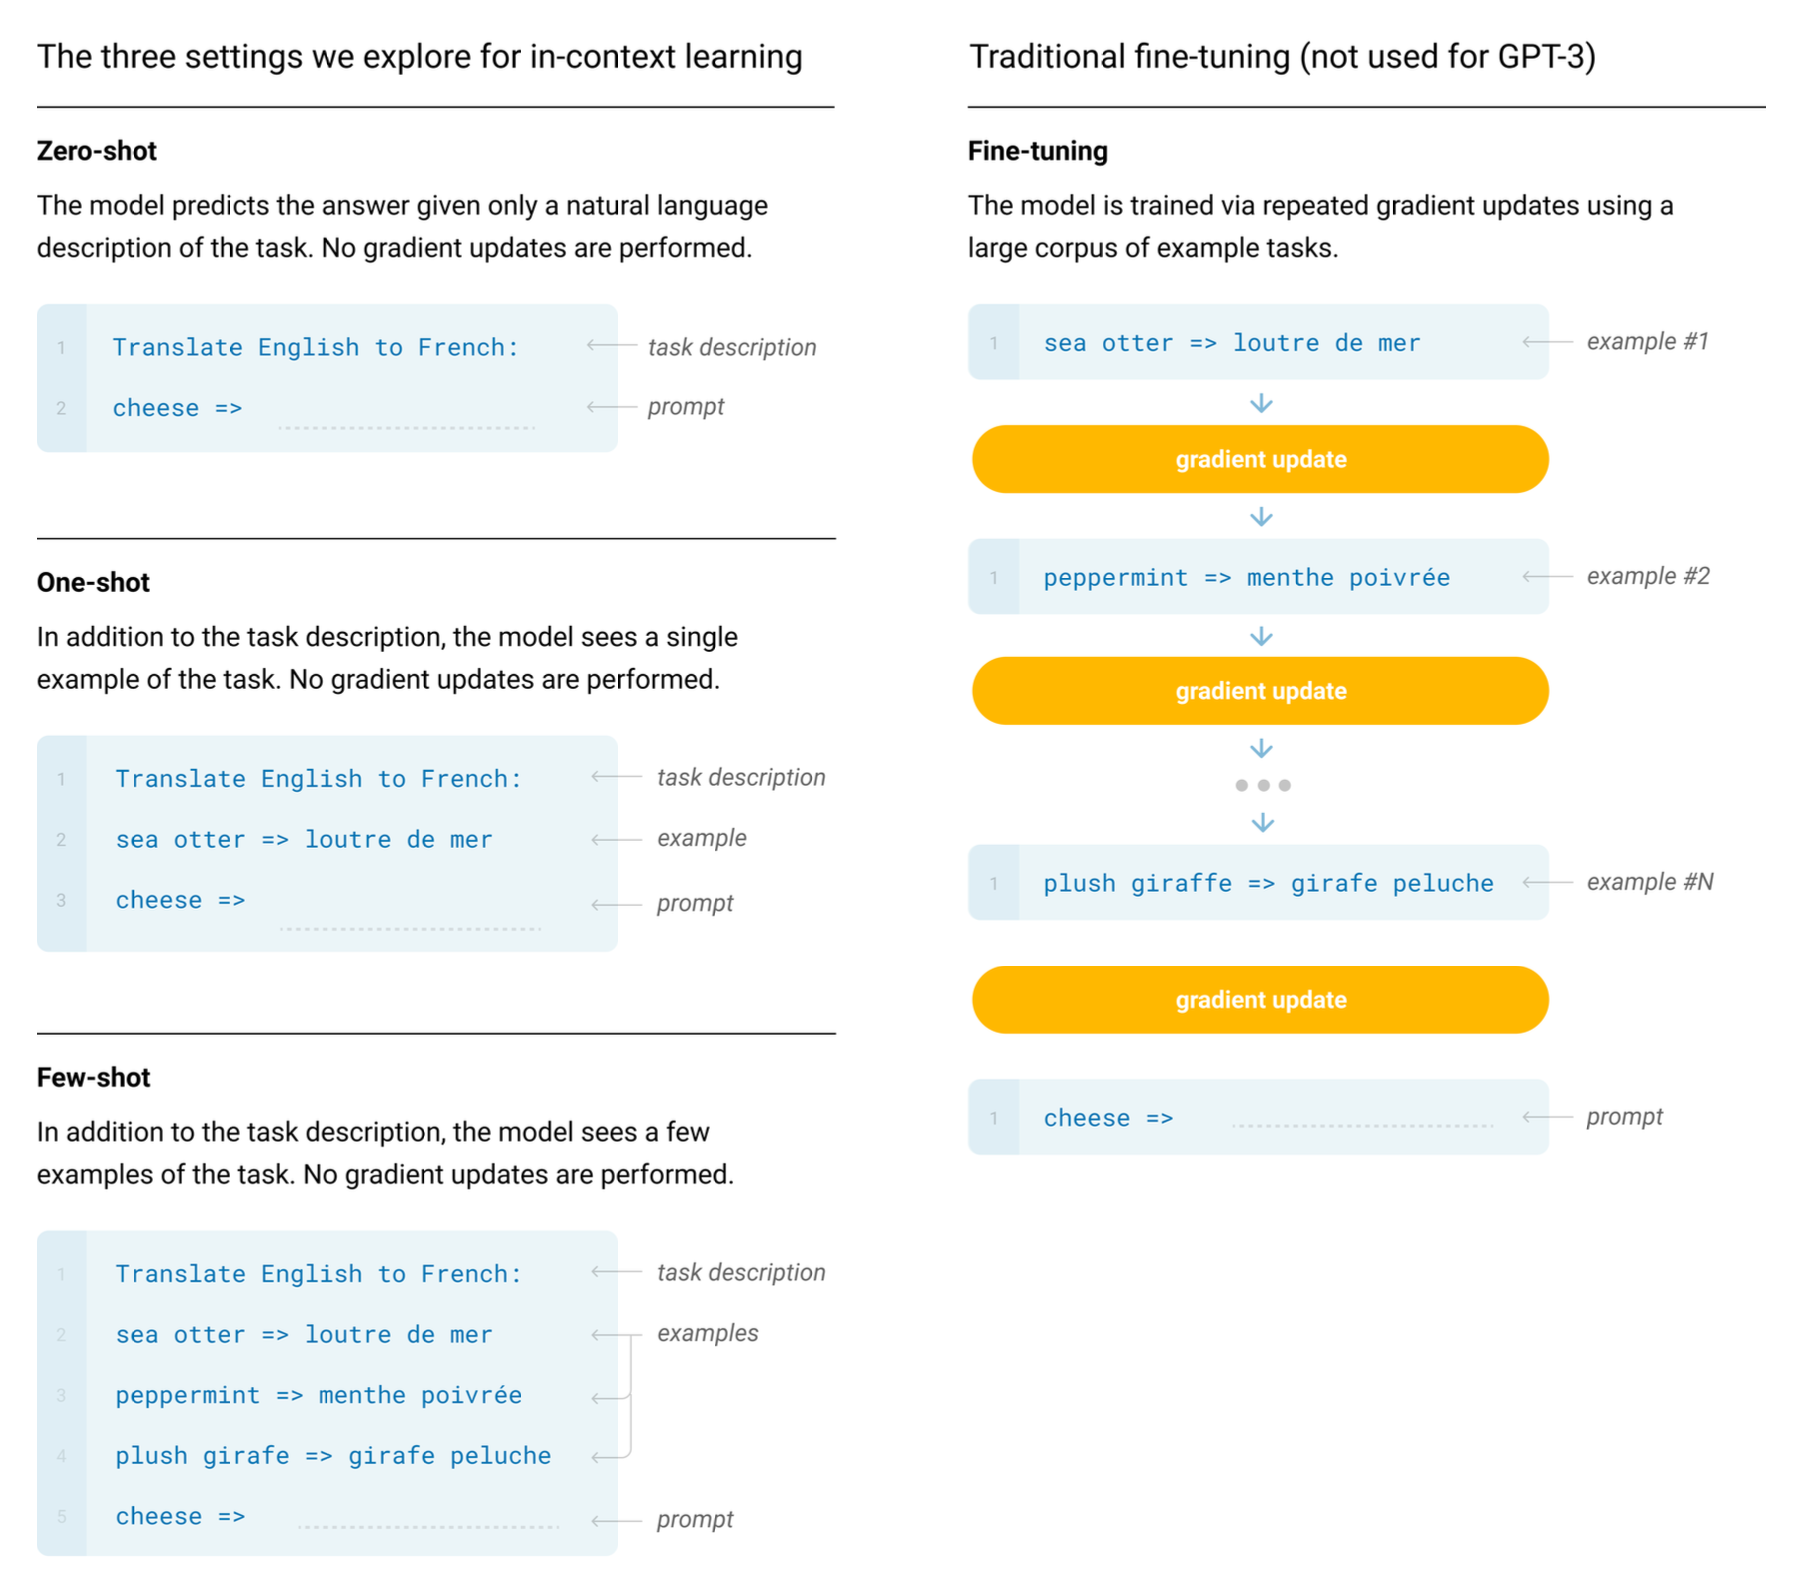
\includegraphics[width=\linewidth]{./fig/gpt3_fig2.png}
  \caption{zero-shot, one-shot, few-shotとfine-tuningの違い\cite{GPT-3}}
  \label{fig:gpt3_example}
\end{figure*}

しかし、GPT-3のような大規模モデルでも、ゼロショット性能はフューショット性能に比べて著しく低いという課題があった。この課題を解決するために、Weiらによって提案されたのが「指示チューニング(Instruction Tuning)」である\cite{Instruction-Tuning}。これは、事前学習済みの言語モデルを、自然言語の「指示(instruction)」として記述された、多数の既存データセットの集合でファインチューニングする手法である。このプロセスでは、入力トークン系列$x = \{x^1, \dots, x^m\}$と正解ラベル$y$からなる教師ありデータセット$C$を用いて、以下の対数尤度を最大化するようにモデルを微調整する。
$$
L_2(C) = \sum_{(x,y) \in C} \log P(y | x^1, \dots, x^m)
$$
ここで、$x$はタスクを説明する指示とタスクの入力を組み合わせたものであり、$y$はモデルが生成すべき正解の出力である。Weiらは、翻訳、質問応答、感情分析など60以上の多様なNLPタスクを用いてこの学習を行い、その結果得られたモデルをFLAN (Finetuned Language Net)と名付けた。

\begin{figure*}[t]
  \centering
  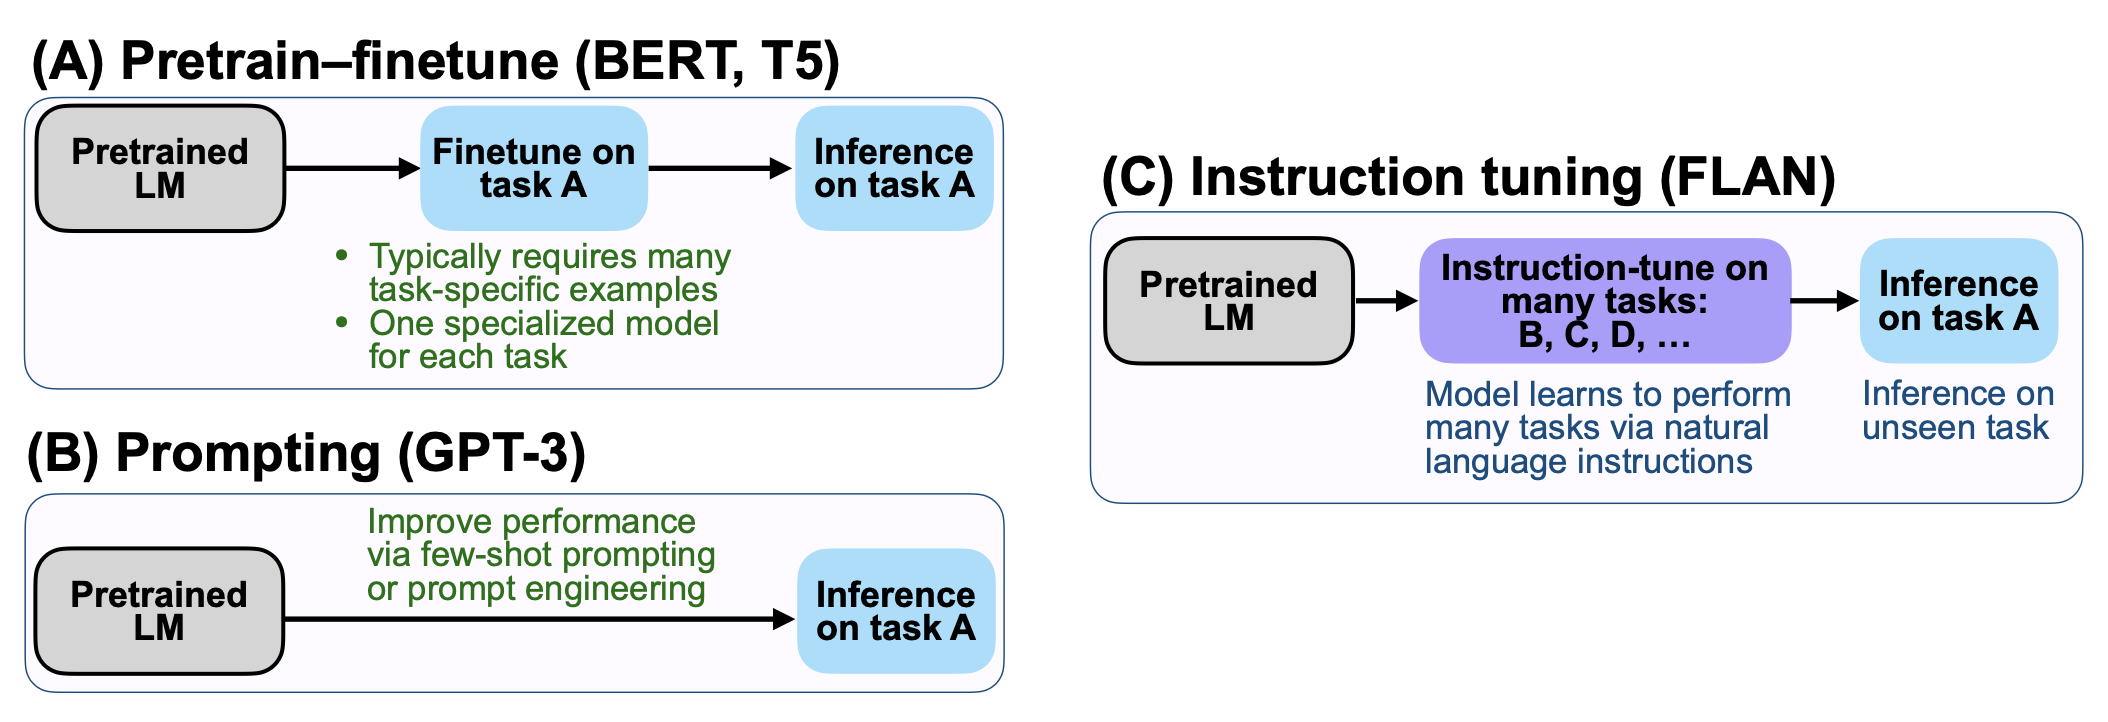
\includegraphics[width=\linewidth]{./fig/flan_fig2.png}
  \caption{FLANの指示チューニングの例\cite{Instruction-Tuning}}
  \label{fig:flan_example}
\end{figure*}

指示チューニングの最大の成果は、学習時には見せていない「未知のタスク」に対するゼロショット性能を大幅に向上させた点にある。論文中のアブレーションスタディにより、この成功の鍵は「モデルの規模(model scale)」と、学習に用いる「タスクの数と多様性(number of finetuning datasets)」であることが明らかにされている。様々なタスクを統一的な指示形式で学習させることで、モデルは個別のタスク解法ではなく、指示に従うという、より一般的で根源的な能力を学習し、高い汎化性能を実現する。

\subsubsection{人間からのフィードバックによる強化学習 (RLHF)}
指示チューニングがモデルにタスクを遂行する能力を付与する一方で、その応答が人間の意図や価値観と一致しているかを保証するものではない。この課題に対し、LLMの挙動をより人間の好みに合致させるためのアライメント技術として、人間からのフィードバックによる強化学習(RLHF: Reinforcement Learning from Human Feedback)が提案された\cite{InstructGPT}。この手法は、特にInstructGPTやChatGPTといったモデルの成功を支える中核技術として知られている。

RLHFのプロセスは、一般的に3つのステップで構成される\cite{InstructGPT}。

\begin{figure*}[t]
  \centering
  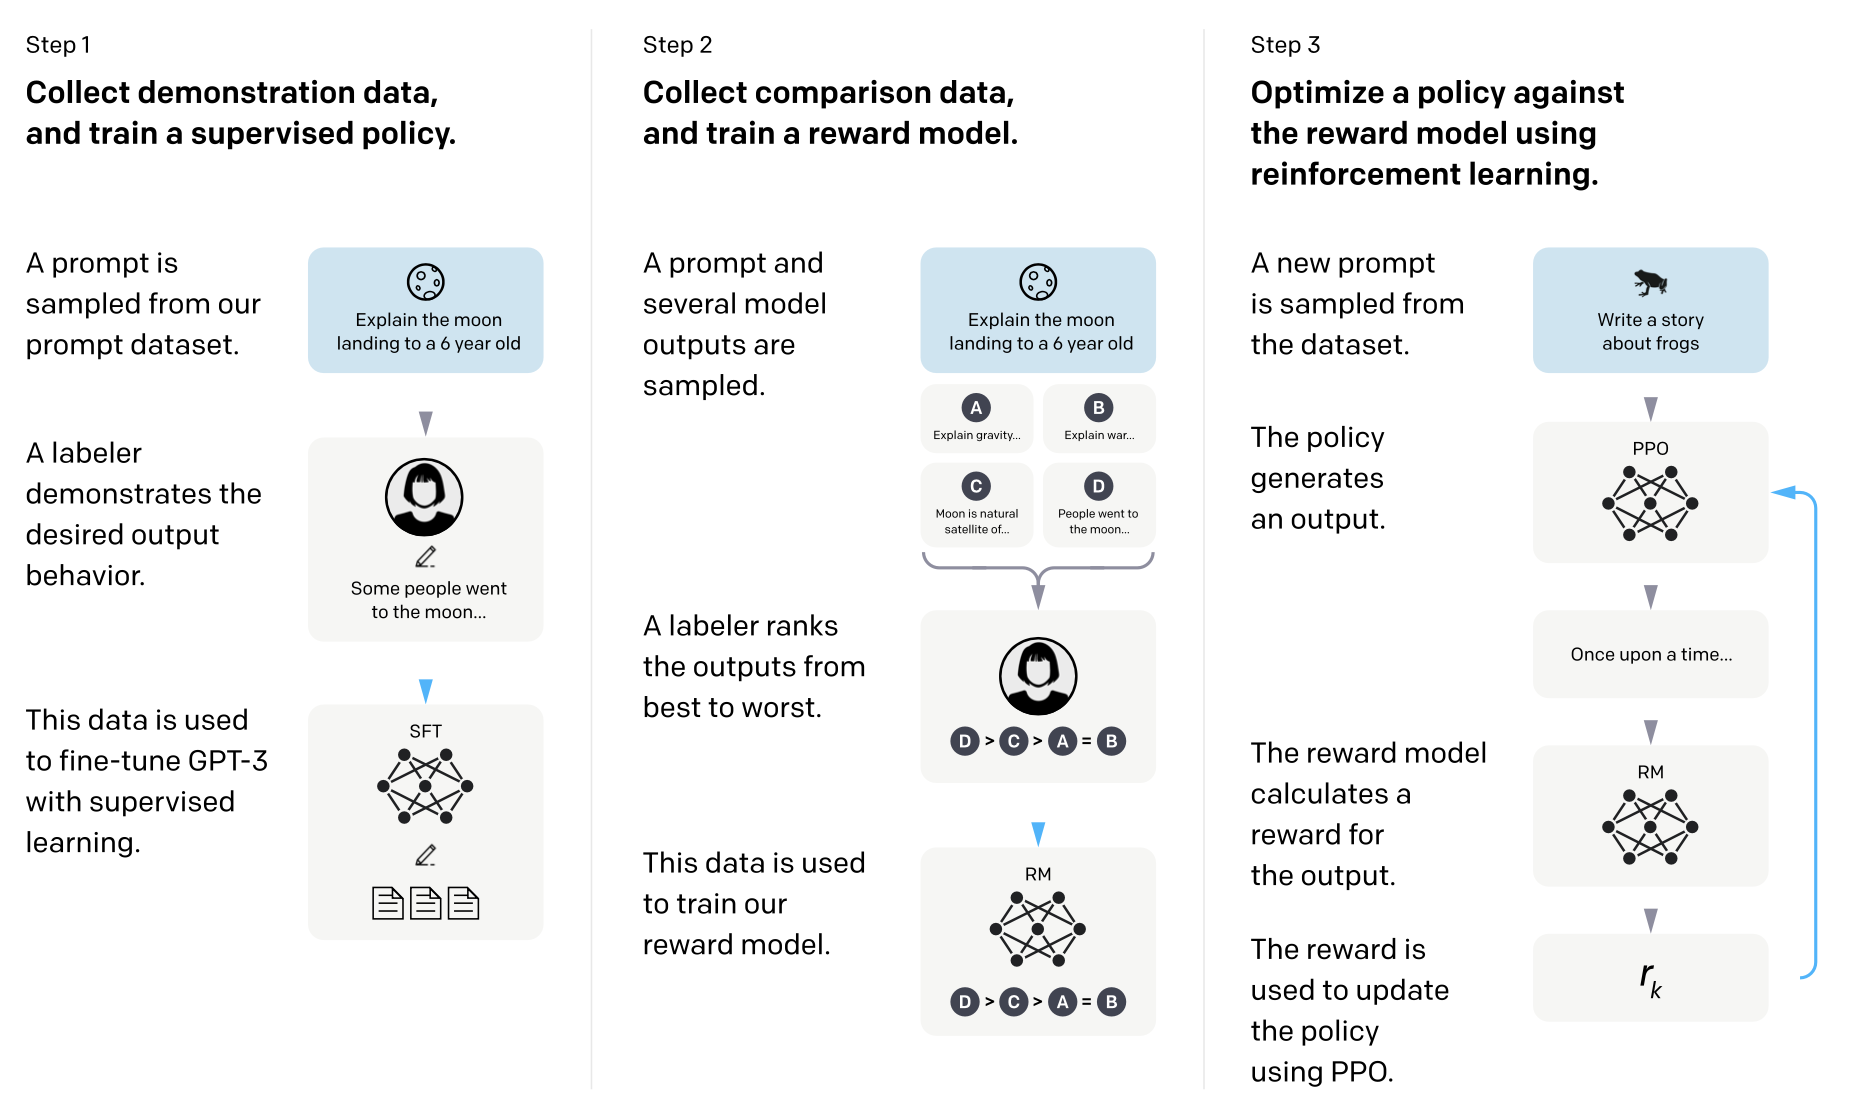
\includegraphics[width=\linewidth]{./fig/rlhf_fig2.png}
  \caption{RLHFのプロセス\cite{InstructGPT}}
  \label{fig:rlhf_process}
\end{figure*}

\begin{enumerate}
    \item \textbf{教師ありファインチューニング (SFT):}
    まず、高品質な指示とそれに対する手本となる応答のデータセットを人間が作成する。事前学習済みの言語モデルを、このデータセットを用いてファインチューニングする。このステップは、モデルに対話や指示応答の基本的な能力を付与し、後の強化学習フェーズにおける初期ポリシー(方策)を形成する役割を持つ。

    \item \textbf{報酬モデルの学習 (Reward Model Training):}
    次に、SFTモデルに同一の指示プロンプトを複数回入力し、複数の異なる応答を生成させる。人間(アノテータ)は、これらの応答を品質や好ましさの観点からランク付けする。この人間による選好データを用いて、どの応答がより好ましいかを予測する「報酬モデル(Reward Model)」を学習させる。

    \item \textbf{強化学習による最適化 (Reinforcement Learning Optimization):}
    最後に、学習した報酬モデルを強化学習の報酬関数として利用する。SFTモデルを初期ポリシーとし、強化学習アルゴリズム(一般的にはPPOが用いられる)を使って、報酬モデルからの報酬が最大化されるように言語モデルのパラメータを更新していく。この際、論文では、ポリシーが元のSFTモデルから大きく逸脱しすぎないようにペナルティを課す項(KLペナルティ)を報酬に加える工夫がなされている\cite{InstructGPT}。これにより、報酬モデルの欠陥を突く「報酬ハッキング」を防ぎつつ、事前学習で獲得した言語能力を維持することができる。
\end{enumerate}
このRLHFの導入により、InstructGPTは元のGPT-3よりもはるかに小規模であるにもかかわらず、人間の評価者から圧倒的に好まれる応答を生成できるようになった\cite{InstructGPT}。この手法は、モデルの出力をより安全で、有用で、人間の意図に沿ったものにするための強力なパラダイムとして確立されている。






\chapter{機械読解データセットSQuAD}
\label{chap:squad_datasets}

本研究は、既存の高品質なデータセットを転用して、新たな評価データセットを自動生成するアプローチを取る。本章では、その基盤となる機械読解データセットの事実上の標準であるSQuADと、本研究で中核的に利用するその日本語版JSQuADについて詳述する。



\section{SQuAD (Stanford Question Answering Dataset)}
\label{sec:squad}

SQuAD (The Stanford Question Answering Dataset) は、Rajpurkarらによって提案された\cite{SQuAD}、機械読解 (Machine Comprehension) の研究を推進するための大規模なデータセットである。その登場以降、質問応答システムの性能を測るための標準ベンチマークとして、この分野の研究に絶大な影響を与えてきた。SQuADの最大の特徴は、その質問応答ペアがクラウドソーシングを通じて人間によって生成されている点にある。具体的には、Wikipediaから選定された記事を文脈(コンテキスト)として用い、クラウドワーカーがその内容に関する質問と、回答となる箇所を文脈中から連続した一部分(スパン)として抜き出すことで、10万件を超える高品質なデータセットを構築している。この「\textbf{extractive question answering}」と呼ばれる形式は、モデルが回答を自由に生成するのではなく、文脈中のどこに答えが書かれているかを正確に特定する能力を求めるものであり、客観的かつ定量的な評価を可能にした。

SQuADにおけるシステムの評価には、主にExact Match (EM)とF1 Scoreの2つの指標が用いられる\cite{SQuAD}。EMはモデルの予測が正解と完全に一致した場合のみを正解とする厳密な指標であり、F1スコアは単語の集合として予測と正解の一致度を測る、より柔軟な指標である。SQuADの登場は、それまでの小規模なデータセットでは不可能だった、深層学習モデルの本格的な学習と評価を可能にし、BERT\cite{BERT}をはじめとする多くの高精度な読解モデルが開発されるきっかけとなり、質問応答研究の発展を大きく加速させた。



\section{JSQuAD (Japanese Stanford Question Answering Dataset)}
\label{sec:jsquad}

JSQuADは、日本語の汎用言語理解ベンチマークJGLUE\cite{JGLUE}の一部として、Kuriharaらによって構築された、日本語の読解能力を評価するための大規模データセットである。その設計思想と構築プロセスは、前節で述べたSQuAD\cite{SQuAD}を基礎としており、日本語における機械読解研究の重要な基盤となっている。構築プロセスはSQuADと同様に、質の高い日本語版Wikipediaの記事をソースとし、クラウドソーシングによって約7万件の質問応答ペアが作成されている。これもまた、回答が文脈中のテキストから抜き出される「extractive」形式を採用している。

\begin{figure*}[t]
  \centering
  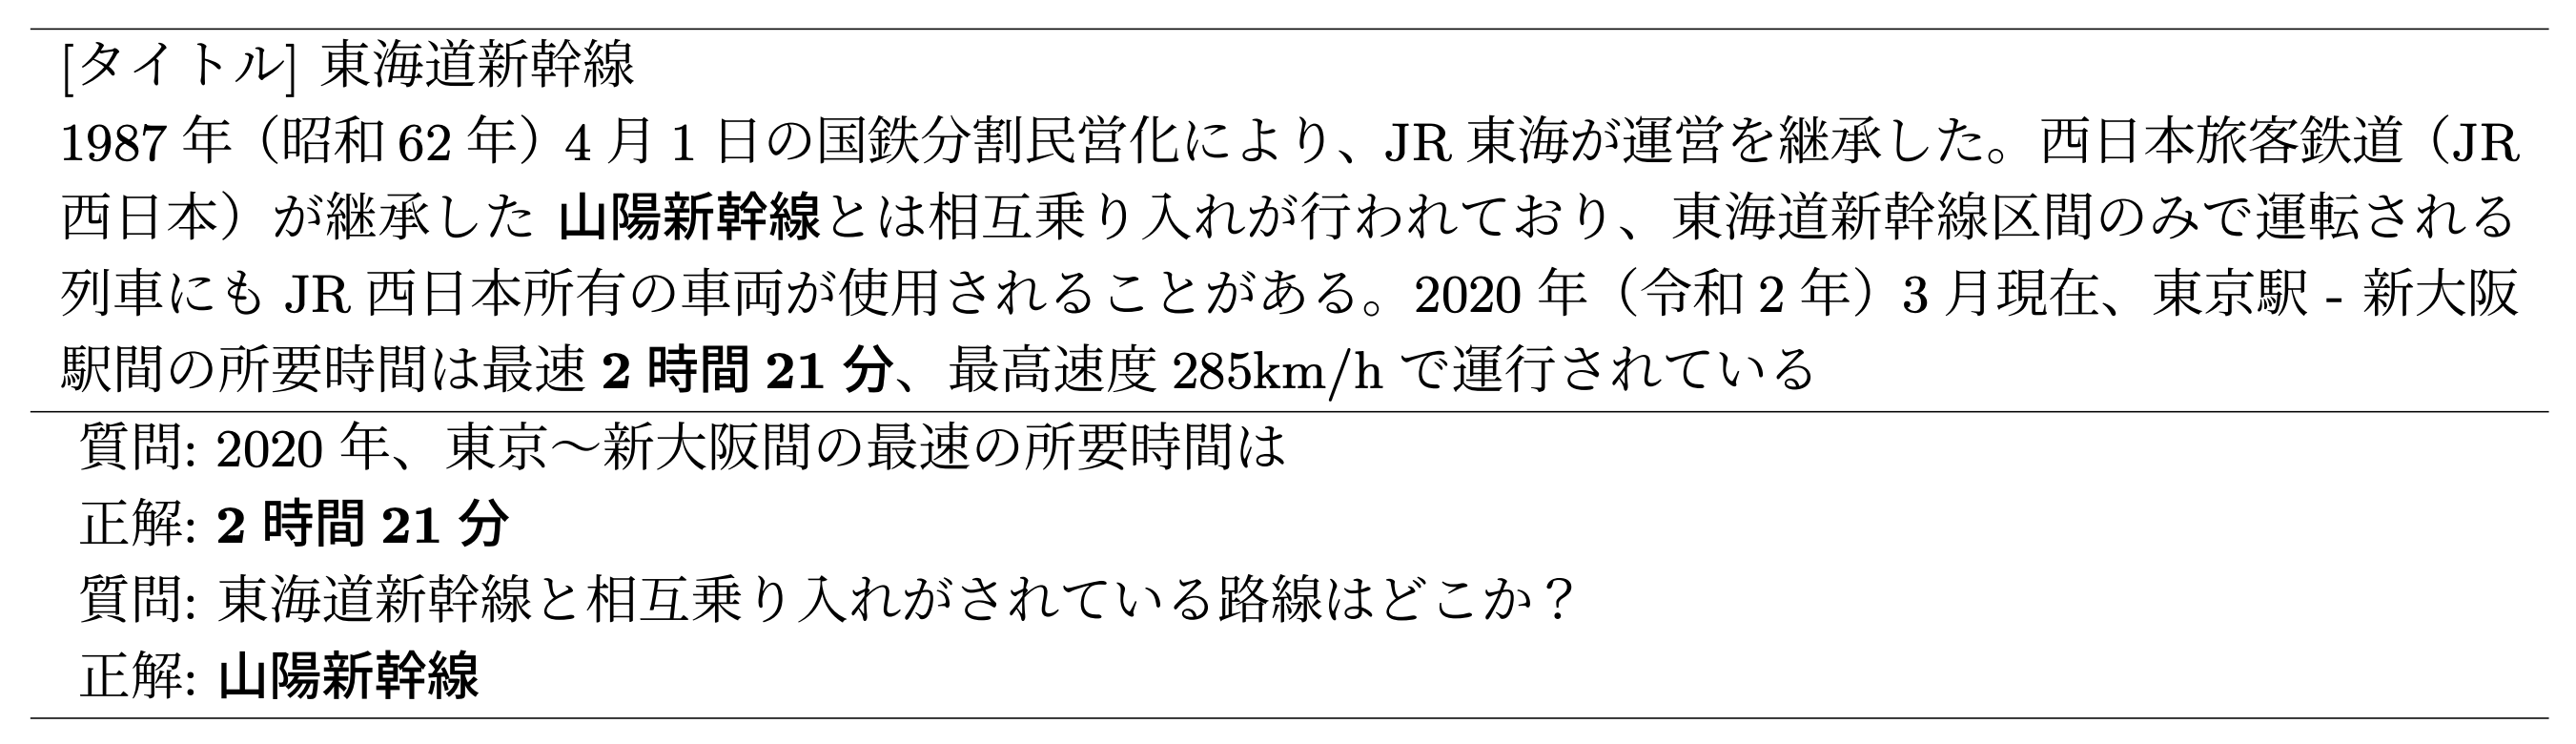
\includegraphics[width=0.9\linewidth]{./fig/jsquad.png}
  \caption{JSQuADのデータ構造例\cite{JGLUE}}
  \label{fig:jsquad_example}
\end{figure*}

評価指標もSQuADと同様にEMとF1スコアが採用されているが、日本語の特性を考慮した重要な工夫がなされている。英語のSQuADではF1スコアを単語単位で計算するが、日本語は単語の区切りが自明ではないため、分かち書きに用いる形態素解析器によって評価値が変動しうる。この問題を回避するため、JSQuADにおけるF1スコアは\textbf{文字単位(character-level)}で計算される\cite{JGLUE}。これにより、形態素解析器の違いに依存しない、安定した評価を実現している。

本研究では、このJSQuADを2つの重要な役割で活用する。第一に、**「教師」としての役割**である。3章で詳述する通り、その高品質な「文脈・質問・回答」の三つ組の入出力構造を転用し、QAペア生成モデルを学習させるための教師データとして用いる。第二に、**「審判」としての役割**である。4章で述べる実験において、自動生成された評価データセットの有効性を評価する上で、JSQuADを人間が作成した基準(ゴールドスタンダード)として利用し、各LLMの性能ランキングを比較するためのベンチマークとする。




\chapter{関連研究}

% \section{SQuAD (Stanford Question Answering Dataset)}
% \label{sec:squad}

% SQuAD (The Stanford Question Answering Dataset) は、Rajpurkarらによって提案された\cite{SQuAD}、機械読解 (Machine Comprehension) の研究を推進するための大規模なデータセットである。その登場以降、質問応答システムの性能を測るための事実上の標準ベンチマークとして、この分野の研究に絶大な影響を与えてきた。SQuADの最大の特徴は、その質問応答ペアがクラウドソーシングを通じて人間によって生成されている点にある。具体的には、まずWikipediaから536本の記事が選定され、文脈(コンテキスト)として用いられる。次に、クラウドワーカー(アノテータ)は、与えられた文脈を読み、その内容に関する質問を最大5つ作成し、その質問に対する回答を必ず文脈中のテキストから連続した一部分(スパン)として抜き出す。このプロセスにより、合計で107,785個の高品質な質問応答ペアが収集された。この「\textbf{extractive question answering}」と呼ばれる形式は、モデルが回答を自由に生成するのではなく、文脈中のどこに答えが書かれているかを正確に特定する能力を求めるものであり、客観的かつ定量的な評価を可能にした。

% SQuADにおけるシステムの評価には、主にExact Match (EM)とF1 Scoreの2つの指標が用いられる\cite{SQuAD}。EMはモデルの予測が正解と完全に一致した場合のみを正解とする厳密な指標であり、F1スコアは単語の集合として予測と正解の一致度を測る、より柔軟な指標である。論文では、SQuADのデータセットが多様な推論能力を要求することも示されており、質問の約20\%は複数文にまたがる情報を統合する必要があるなど、高度な推論を必要とする。SQuADの登場は、それまでの小規模なデータセットでは不可能だった、深層学習モデルの本格的な学習と評価を可能にし、BERT\cite{BERT}をはじめとする多くの高精度な読解モデルが開発されるきっかけとなり、質問応答研究の発展を大きく加速させた。



% \section{JSQuAD (Japanese Question Answering Dataset)}
% \label{sec:jsquad}

% JSQuADは、日本語の汎用言語理解ベンチマークJGLUE\cite{JGLUE}の一部として、Kuriharaらによって構築された、日本語の読解能力を評価するための大規模データセットである。その設計思想と構築プロセスは、先行するSQuAD\cite{SQuAD}を基礎としており、日本語における機械読解研究の重要な基盤となっている。構築プロセスはSQuADと同様に、質の高い日本語版Wikipediaの記事をソースとし、クラウドソーシングによって約7万件の質問応答ペアが作成されている。これもまた、回答が文脈中のテキストから抜き出される「extractive」形式を採用している。

% 評価指標もSQuADと同様にEMとF1スコアが採用されているが、日本語の特性を考慮した重要な工夫がなされている。英語のSQuADではF1スコアを単語単位で計算するが、日本語は単語の区切りが自明ではないため、分かち書きに用いる形態素解析器によって評価値が変動しうる。この問題を回避するため、JSQuADにおけるF1スコアは\textbf{文字単位(character-level)}で計算される\cite{JGLUE}。これにより、形態素解析器の違いに依存しない、安定した評価を実現している。

% 本研究では、このJSQuADを2つの重要な役割で活用する。第一に、**「教師」としての役割**である。3章で詳述する通り、その高品質な「文脈・質問・回答」の三つ組の入出力構造を転用し、QAペア生成モデルを学習させるための教師データとして用いる。第二に、**「審判」としての役割**である。4章で述べる実験において、自動生成された評価データセットの有効性を評価する上で、JSQuADを人間が作成した基準(ゴールドスタンダード)として利用し、各LLMの性能ランキングを比較するためのベンチマークとする。
% \begin{figure*}[t]
%   \centering
%   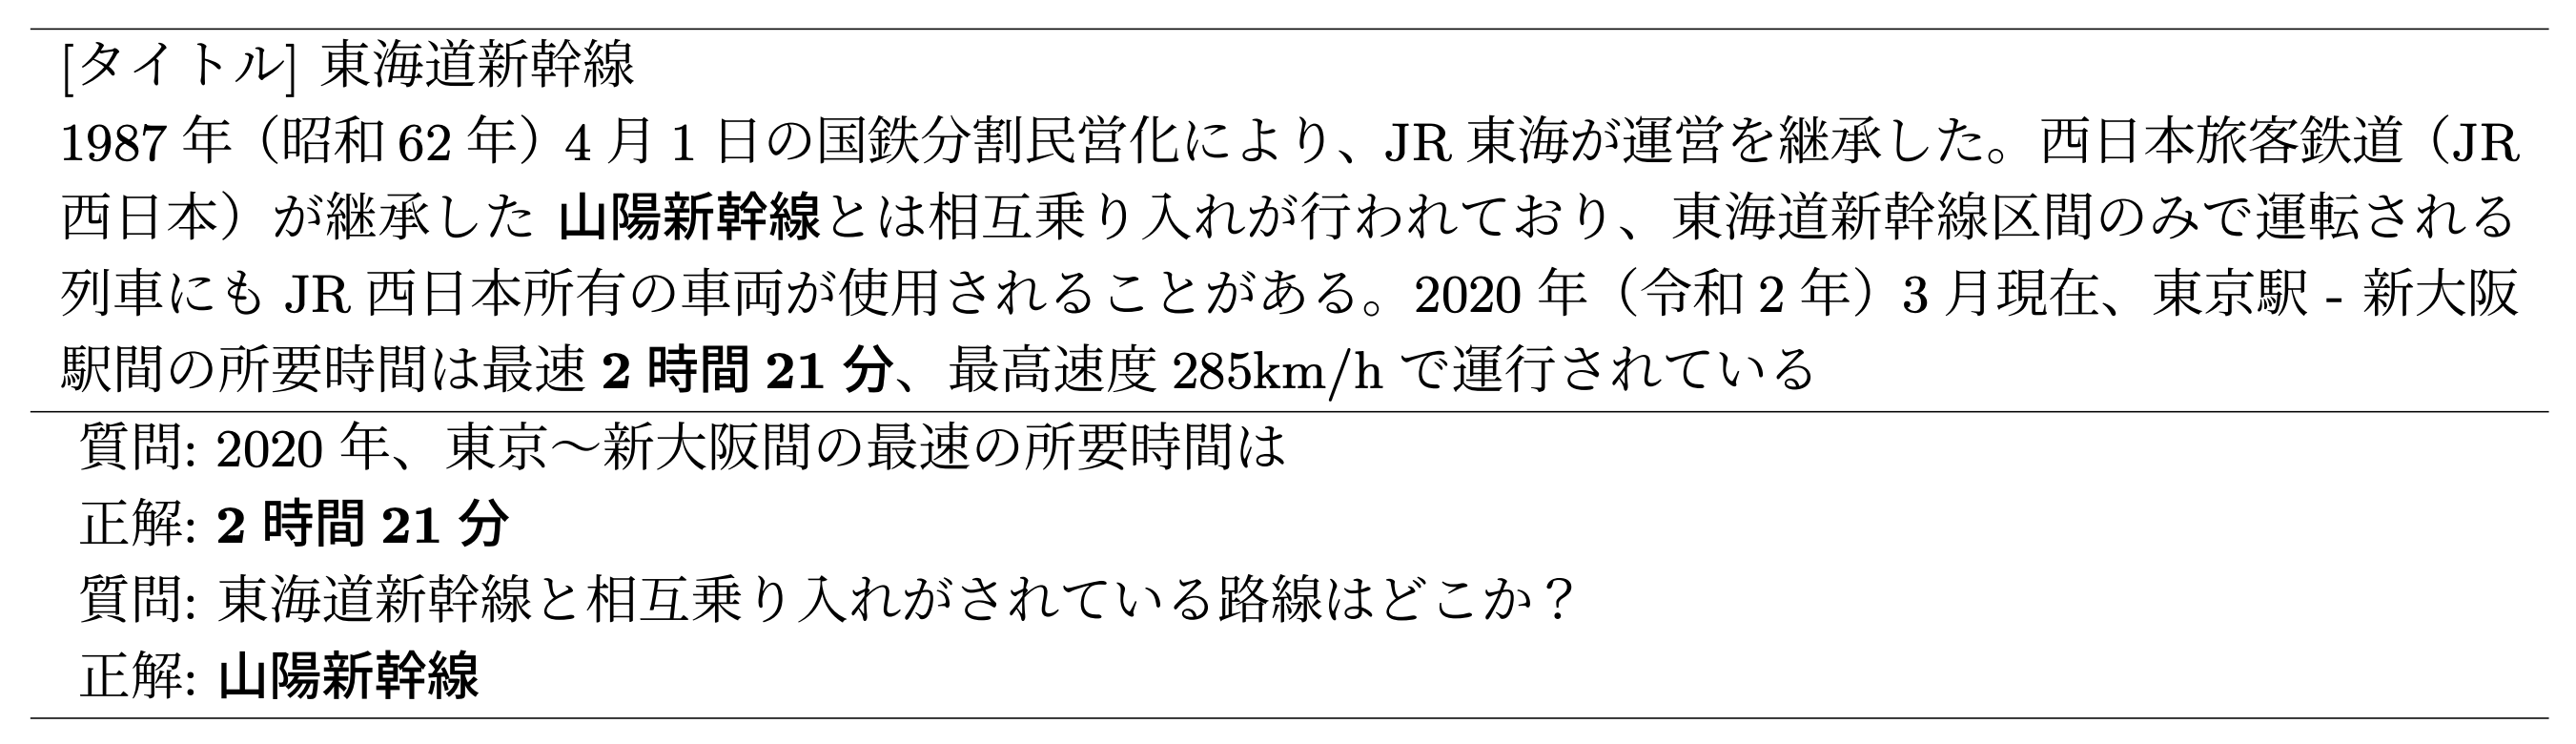
\includegraphics[width=\linewidth]{./fig/jsquad.png}
%   \caption{JSQuADのデータ構造例\cite{JGLUE}}
%   \label{fig:jsquad_example}
% \end{figure*}



% \section{指示チューニング (Instruction Tuning)}
% 指示チューニングは、大規模言語モデル(LLM)の能力を飛躍的に向上させた重要な技術の一つである。このアプローチの根底には、BrownらがGPT-3で示した「文脈内学習(in-context learning)」の概念がある。文脈内学習とは、モデルの重みを更新(ファインチューニング)することなく、推論時にプロンプトとして少数のタスク例(デモンストレーション)を与えるだけで、モデルがそのタスクを遂行する能力を指す。この能力は、与える例の数に応じて「ゼロショット(zero-shot)」「ワンショット(one-shot)」「フューショット(few-shot)」として区別され、特にモデルの規模が大きくなるほど、文脈内の例からタスクを学習する効率が劇的に向上することが示された。

% \begin{figure*}[t]
%   \centering
%   \includegraphics[width=\linewidth]{./fig/gpt3\_fig2.png}
%   \caption{zero-shot, one-shot, few-shotとfine-tuningの違い\cite{GPT-3}}
%   \label{fig:gpt3_example}
% \end{figure*}

% しかし、GPT-3のような大規模モデルでも、ゼロショット性能はフューショット性能に比べて著しく低いという課題があった。この課題を解決するために、Weiらによって提案されたのが「指示チューニング(Instruction Tuning)」である。これは、事前学習済みの言語モデルを、自然言語の「指示(instruction)」として記述された、多数の既存データセットの集合でファインチューニングする手法である。Weiらは、翻訳、質問応答、感情分析など60以上の多様なNLPデータセットを収集し、それぞれに複数の指示テンプレート(例:「この映画レビューの感情はポジティブですか、ネガティブですか?」)を作成した。そして、この大規模な指示データセットの混合物でモデルを学習させ、その結果得られたモデルをFLAN (Finetuned Language Net)と名付けた。

% \begin{figure*}[t]
%   \centering
%   \includegraphics[width=\linewidth]{./fig/flan\_fig2.png}
%   \caption{FLANの指示チューニングの例\cite{Instruction-Tuning}}
%   \label{fig:flan_example}
% \end{figure*}

% 指示チューニングの最大の成果は、学習時には見せていない「未知のタスク」に対するゼロショット性能を大幅に向上させた点にある。FLANは、より大規模なGPT-3のゼロショット性能を多くのタスクで上回り、いくつかのタスクではフューショット性能すら凌駕した。論文中のアブレーションスタディにより、この成功の鍵は「モデルの規模(model scale)」と、学習に用いる「タスクの数と多様性(number of finetuning datasets)」であることが明らかにされている。様々なタスクを統一的な指示形式で学習させることで、モデルは個別のタスク解法ではなく、指示に従うという、より一般的で根源的な能力を学習し、高い汎化性能を実現する。このパラダイムは、後の多くの対話型・指示追従型LLM開発の基礎となっている。



\section{Self-Instruct}
\label{sec:self-instruct}

Self-Instructは、Wangらによって提案された\cite{Self-Instruct}、大規模言語モデル(LLM)自身を用いて、そのモデルの指示追従能力を向上させるための大規模な指示データセットを生成するフレームワークである。このアプローチは、人間による大規模なアノテーションコストをかけずに、既存の事前学習済みLLMの能力を最大限に引き出すことを目的としている。

\begin{figure*}[t]
  \centering
  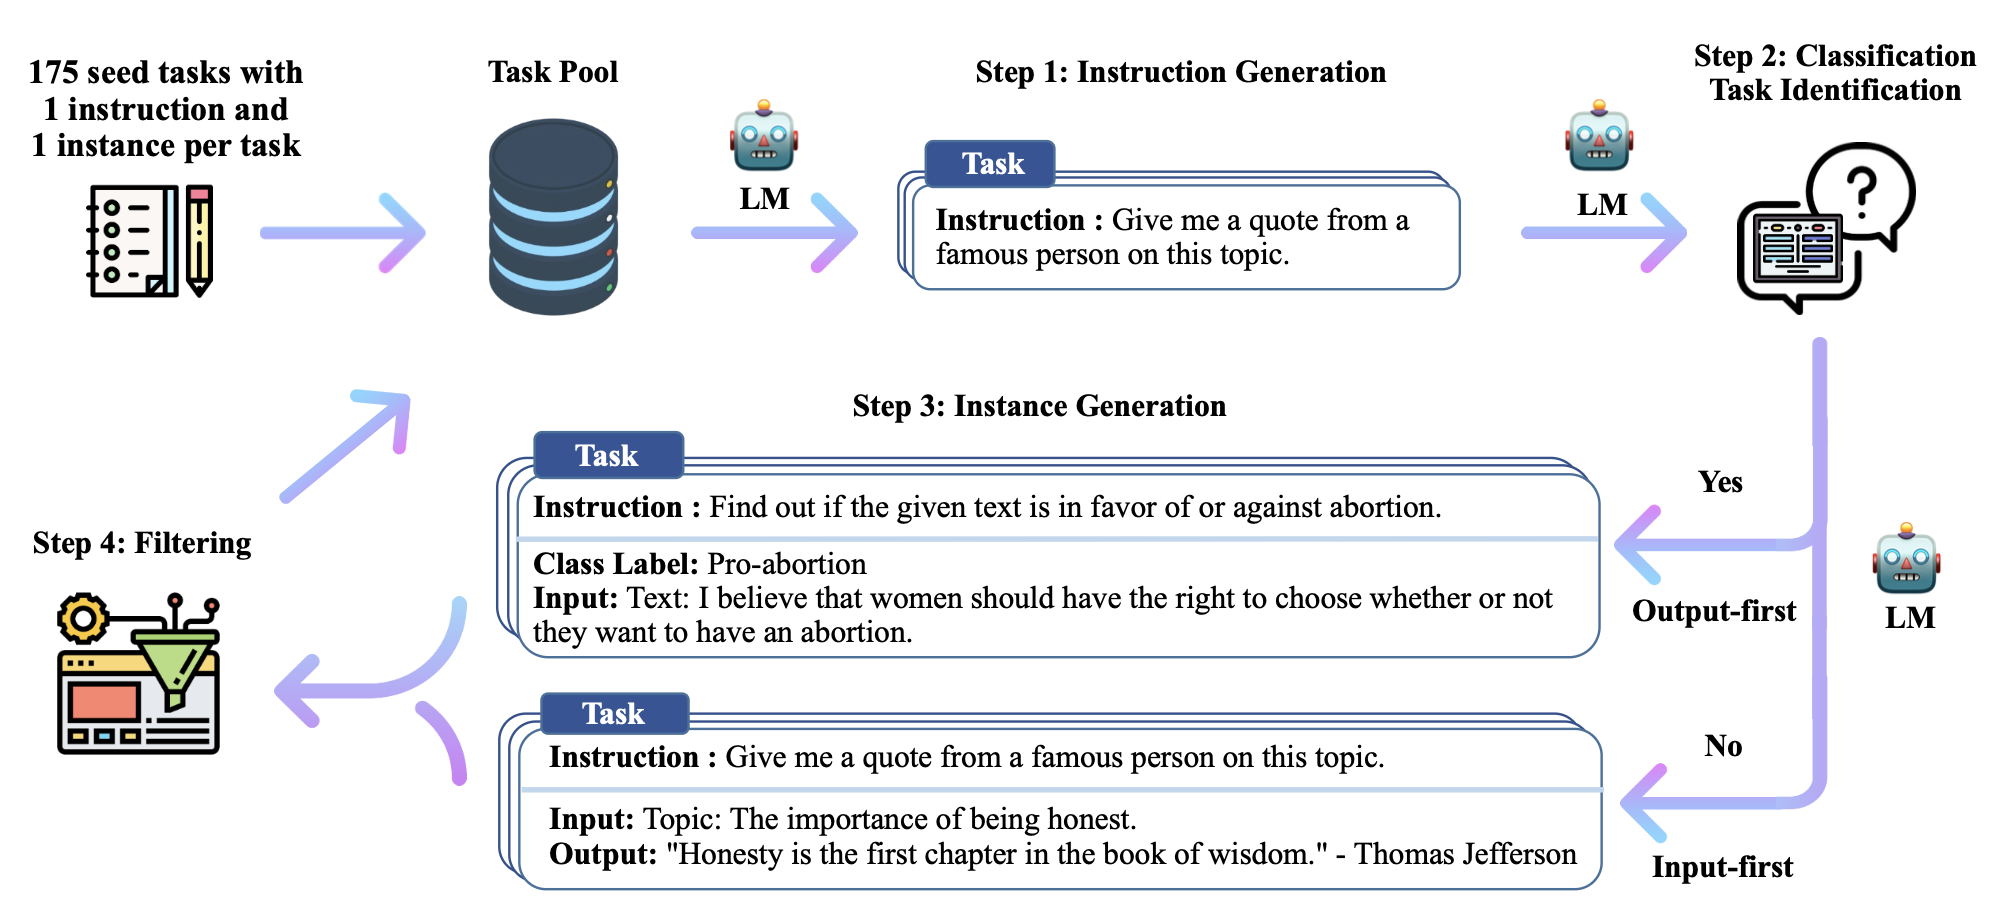
\includegraphics[width=\linewidth]{./fig/self-instruct_fig1.png}
  \caption{Self-Instructのデータ生成プロセス\cite{Self-Instruct}}
  \label{fig:self_instruct_example}
\end{figure*}

Self-Instructのプロセスは、人間が作成した少数の多様な指示(論文では175個)を「シードセット」として用いることから始まる。このシードセットを基に、LLM(論文ではGPT-3)に対して自己生成的なプロンプティングを行い、新たな指示を生成させる。具体的には、既存の指示を数例提示し、「これらに似た新しい指示を生成してください」といった形でLLMに問いかける。次に、生成された新しい指示が、既存の指示と類似しすぎていないか、あるいは不適切な内容でないかをフィルタリングする。そして、フィルタリングを通過した質の高い新規指示に対して、再度LLMを用いて、その指示を解くための具体的なインスタンス(入力と出力のペア)を生成させる。この一連の「指示生成→フィルタリング→インスタンス生成」のパイプラインを繰り返すことで、指示データセットを大規模に拡張していく。

この研究の重要な貢献は、このようにして自動生成されたデータセット(論文では52,000件以上)で、元の事前学習済みLLMをファインチューニングすることにより、その指示追従能力が大幅に向上することを示した点にある。実際、ファインチューニング後のモデルは、元のGPT-3の性能を上回り、人間による評価では当時最高性能であった`text-davinci-001`に匹敵する結果を示した\cite{Self-Instruct}。

本研究のアプローチは、LLMを用いて学習データを合成するという点でSelf-Instructと共通している。しかし、両者には明確な差異が存在する。Self-Instructが少数のシードから多様なタスクの指示を**ゼロから生成**し、モデルの**汎用的な指示追従能力**の向上を目指すのに対し、本研究は既存の高品質な読解データセット(JSQuAD)の**データ構造を転用**し、**特定の目的(評価データ生成)**に特化したデータを生成する。特に、本研究のアプローチは、常に信頼できる「文脈」に事実を基づかせることで、Self-Instructで課題となりうるハルシネーションを原理的に抑制する設計となっている点が異なる。



\section{指示事前学習 (Instruction Pre-Training)}
\label{sec:instruction_pre-training}

指示事前学習(Instruction Pre-Training)は、Chengらによって提案された\cite{Instruction Pre-Training}、言語モデルの**事前学習**段階そのものに、教師ありの指示データを大規模に組み込む新しいフレームワークである。従来、LLMの事前学習はラベルなしの生コーパスのみを用いる自己教師あり学習(Vanilla Pre-Training)が主流であった。これに対し、本手法では事前学習の段階からモデルに多様なタスクを解く能力を学習させることを目的とする。

そのプロセスは、まず「指示シンセサイザ(instruction synthesizer)」と呼ばれるモデルを用いて、生コーパスの内容に基づいた「指示と応答(instruction-response)」のペアを大量に自動生成する。次に、元の生コーパスと生成された指示応答ペアを組み合わせた「指示拡張コーパス(instruction-augmented corpora)」を構築し、これを最終的な事前学習データとして用いる。このアプローチの核心は、生コーパスの内容に事実を基づかせた(Fact-Grounded)教師あり信号を、事前学習の段階でモデルに与える点にある。

\begin{figure*}[t]
  \centering
  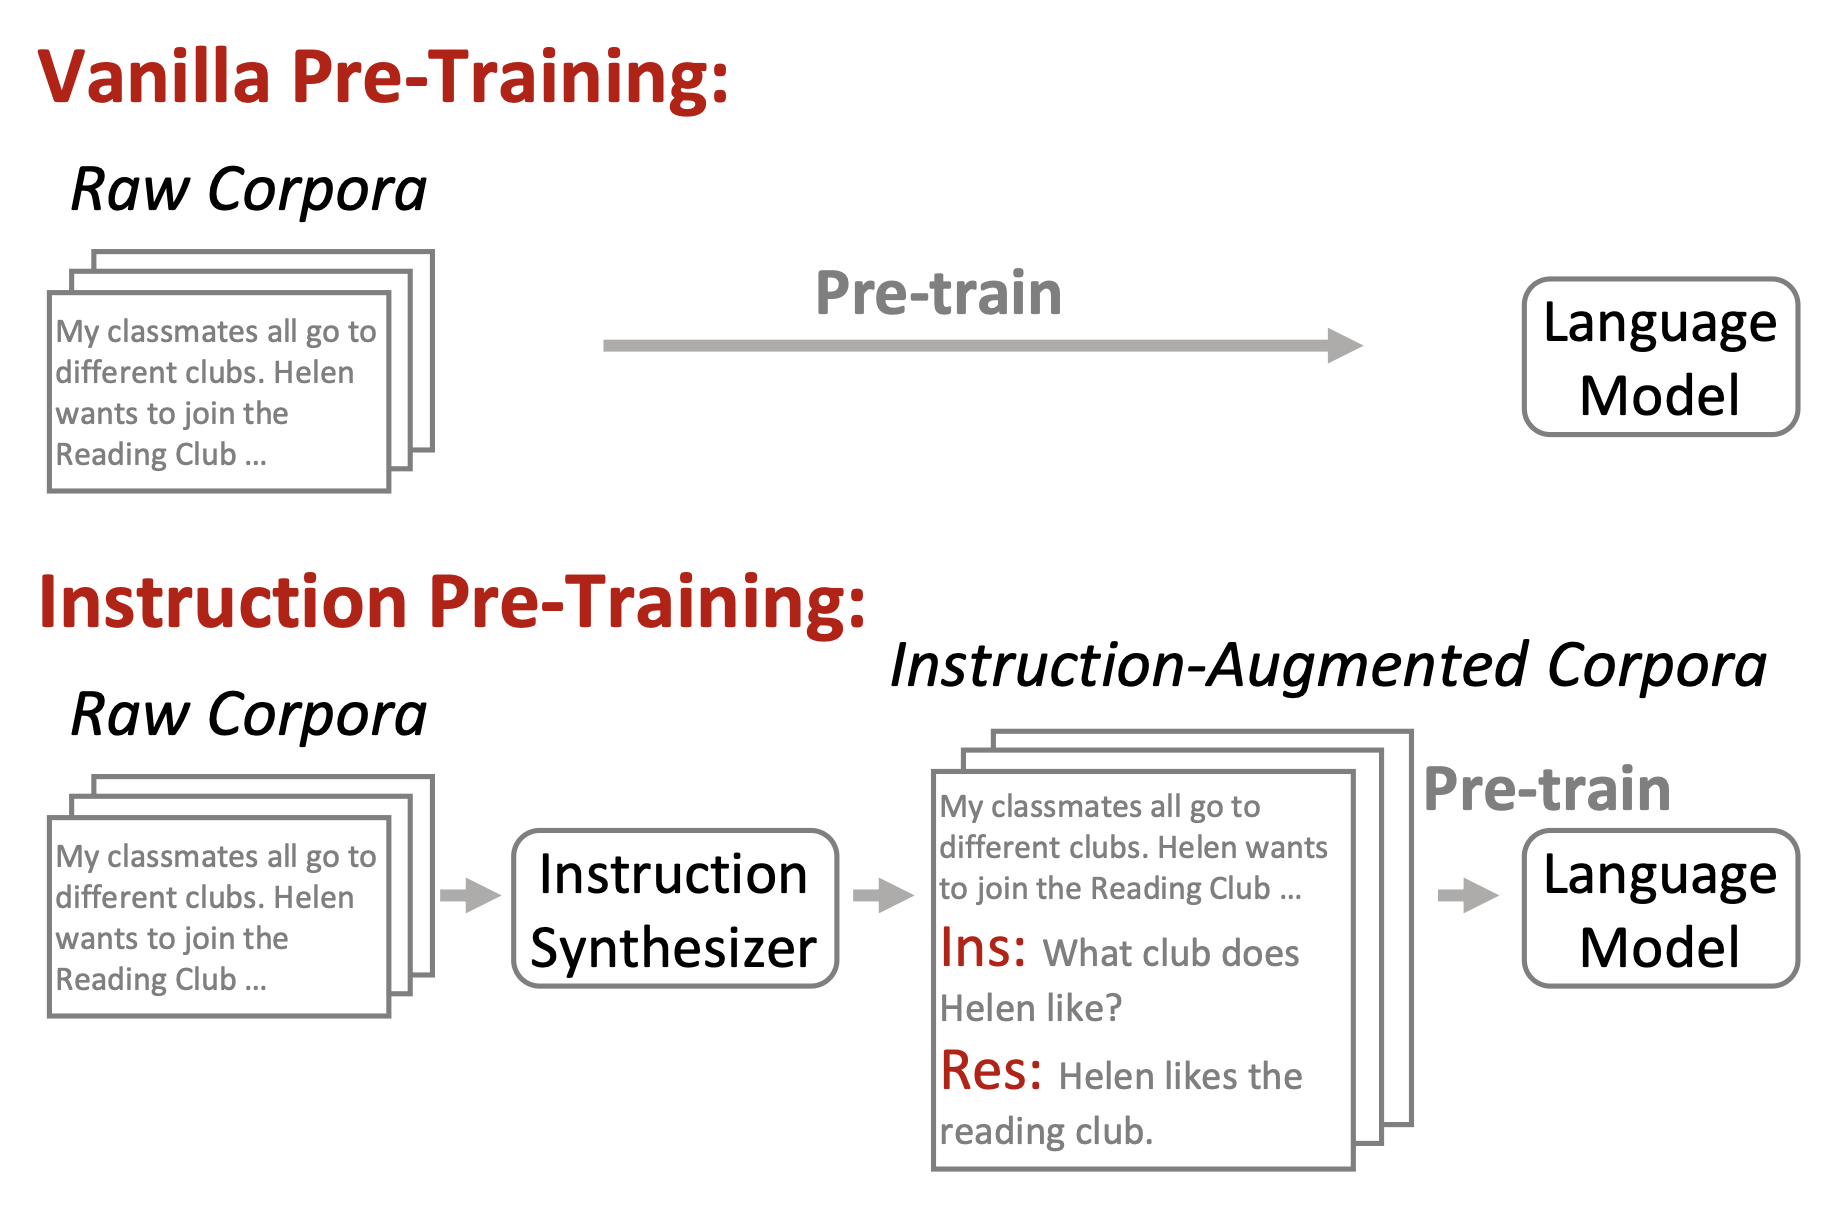
\includegraphics[width=\linewidth]{./fig/instruction-pretraining_fig1.png}
  \caption{一般的な事前学習と指示事前学習の違い\cite{Instruction Pre-Training}}
  \label{fig:instruction_pretraining_example}
\end{figure*}

この指示シンセサイザは、SQuADやHotpotQAなど多様な既存データセットを「文脈から指示と応答のペアを生成する」という形式に変換して学習データとし、オープンソースの言語モデル(例:Mistral-7B)をファインチューニングすることで構築される\cite{Instruction Pre-Training}。このアプローチは、本研究における「JSQuADのデータ構造を組み替えて指示チューニングデータを作成する」という着想と共通点が多い。しかし、本論文がモデルの汎用的な能力向上を目指して**事前学習**の段階で指示データを導入するのに対し、本研究では**評価用データセットの生成**という特定の目的のために**ファインチューニング**段階で指示チューニングを活用する点で、目的と適用段階が明確に異なる。

論文では、この手法で事前学習されたモデルは、従来のモデルを上回る性能を示すだけでなく、その後の指示チューニングからもより大きな恩恵を受けることが示されている\cite{Instruction Pre-Training}。これは、事前学習とファインチューニングのタスク形式が近接することで、両段階の移行がよりスムーズになるためだと考察されている。










\chapter{提案手法}
本章では、信頼性の高い日本語評価データを自動生成するための提案手法について詳述する。

\section{概要}
本研究では、ハルシネーションを抑制し、事実に基づいた評価データを生成するため、**文脈情報に基づきQAペアを生成する**アプローチを採用する。具体的な手法として、日本語の読解データセットであるJSQuADを転用した**指示チューニング**を主軸に据え、その有効性をベースライン手法と比較することで検証する。

\section{テストデータ生成アプローチ}
テストデータを生成するモデル(生成モデル)として、日本語処理能力に優れた`tokyotech-llm/Llama-3.1-Swallow-8B-Instruct-v0.3`\cite{Fujii:COLM2024}を用いる。このモデルにテストデータを生成させるアプローチとして、以下の3つを実装し、比較する。

\subsection{Zero-Shot推論}
Zero-Shot推論は、追加の学習や具体例の提示なしに、一般的な指示のみでタスクを遂行させる最も基本的なアプローチである。本研究では、「この文章に基づいて質問と回答を生成してください」といった指示プロンプトと文脈情報を生成モデルに与え、QAペアを生成させる。これは、後述する手法の有効性を測る上でのベースラインとして機能する。

\subsection{Few-Shot推論}
Few-Shot推論は、プロンプト内に少数のQA生成の模範例を提示する手法である。本研究では、JSQuADから抽出した10個の「文脈、質問、回答」のペアを例としてプロンプトに含める。これにより、生成モデルがタスクをより正確に理解し、質の高いテストデータを生成することを期待する。

\subsection{指示チューニングによる生成}
本研究の主軸となるアプローチが、指示チューニング\cite{Instruction-Tuning}の活用である。この手法の独創的な核心は、高品質な読解データセットであるJSQuAD\cite{JSQuAD}を、QAペア生成モデルの学習用途として効果的に活用する点にある。

本来、JSQuADは「文脈」と「質問」を入力とし、「回答」を予測する読解タスク用に設計されている。本研究ではこの入出力構造を意図的に組み替え、「文脈」のみを入力とし、対応する「質問と回答のペア」全体を出力するようにタスクを再定義した。この「発想の転換」により、読解モデル評価用のデータセットを、QAペア生成モデルの学習用教師データとして活用することが可能となる。これにより、モデルは文脈から適切な問いと答えを創出する能力を直接的に学習し、学習後には未知の文脈を入力するだけで、その内容に基づいたQA形式の評価データを生成できるようになる。

\section{有効性の評価フレームワーク}
上記のアプローチで生成した各評価データセットの有効性をテストするため、統一された評価フレームワークを構築した。性能評価の基準(ベースライン)として、人間が作成したJSQuADの検証データセットを本来の読解タスクとして用いる。この基準データセットを12種類のオープンソースLLM群に解かせ、それぞれの正解率(回答の完全一致率)を基に「モデル性能の基準ランキング」を算出する。次に、自動生成した各評価データセットを用いて同様に12モデルの性能ランキングをそれぞれ算出する。最終的に、「基準ランキング」と「自動生成データによるランキング」との間にどの程度の相関があるかを、スピアマンの順位相関係数($\rho$)を用いて定量的に評価する。この$\rho$値が1に近いほど、自動生成された評価データが、人手によるベンチマークと同等の信頼性を持つ評価軸として機能することを示す。

\chapter{実験}

\section{目的}
本実験の目的は、3章で述べた提案手法の有効性を実証することにある。具体的には、以下の3つの生成アプローチで作成したテストデータセットが、人間製ベンチマーク(JSQuAD)によるLLMの性能ランキングをどの程度忠実に再現できるかを、スピアマンの順位相関係数を用いて定量的に比較・評価する。
\begin{itemize}
    \item Zero-Shot推論
    \item 10-Shot推論
    \item 指示チューニング(提案手法)
\end{itemize}

\section{実験設定}
表\ref{tab:exp_setting}に本実験の主要な設定を示す。テストデータ生成には、日本語に特化した`tokyotech-llm/Llama-3.1-Swallow-8B-Instruct-v0.3`\cite{Fujii:COLM2024}を用いた。有効性評価の対象には、Gemma、Qwen、aya-23-8Bなど、性能や特性が異なる12種類のオープンソースLLMを選定した。これらのモデルは推論用に4bit量子化されたgguf形式に変換して使用する。

\begin{table}[h]
  \centering
  \caption{主要な実験設定}
  \label{tab:exp_setting}
  \begin{tabularx}{0.9\linewidth}{lX}
  \hline
  項目       & 内容 \\
  \hline
  生成モデル   & `tokyotech-llm/Llama-3.1-Swallow-8B-Instruct-v0.3` \\
  学習データ   & JSQuAD (日本語版SQuAD) \\
  比較手法   & Zero-Shot推論、10-Shot推論 \\
  評価対象モデル & オープンソースLLM 12種類 (4bit量子化) \\
  基準データ   & JSQuAD検証データセット \\
  評価指標     & スピアマンの順位相関係数 ($\rho$) \\
  \hline
  \end{tabularx}
\end{table}

\section{実験結果}
人間製データであるJSQuADを用いて12の対象モデルの性能を評価し、これを基準ランキングとした。次に、Zero-Shot推論、10-Shot推論、そして提案手法である指示チューニングの3つのアプローチでテストデータを生成し、それぞれで対象モデルの性能ランキングを算出した。基準ランキングと各生成データによるランキングとのスピアマンの順位相関係数($\rho$)を表\ref{tab:rho_summary_main}にまとめる。

\begin{table}[h]
  \centering
  \caption{各生成アプローチと順位相関係数の比較}
  \label{tab:rho_summary_main}
  \begin{tabular}{lc}
  \hline
  生成アプローチ       & 順位相関係数 ($\rho$) \\
  \hline
  Zero-Shot 推論       & 0.6364 \\
  10-Shot 推論         & 0.7622 \\
  指示チューニング(提案手法) & \textbf{0.8741} \\
  \hline
  \end{tabular}
\end{table}

\section{考察}
表\ref{tab:rho_summary_main}が示す通り、相関係数はZero-Shot推論の$\rho=0.6364$から、Few-Shot推論で$\rho=0.7622$へ、そして指示チューニングでは$\rho=0.8741$へと段階的に向上した。この傾向は、生成モデルへの指示をより具体的に、かつタスクに特化させるほど、生成されるテストデータセットの信頼性が向上することを示唆している。

特に、本研究の主軸である指示チューニングアプローチが高い相関を達成したことは、JSQuADのデータ構造を組み替えて学習させるという本手法の有効性を強く裏付けている。これにより、人間が作成したベンチマークの評価軸を極めて忠実に再現可能であることが実証された。

なお、自動生成データを用いた際の各モデルの絶対的な正解率は、人間製データで評価した際よりも全体的に低下する傾向が見られた。これは生成された問題の難易度や表現の揺れに起因すると考えられる。しかし、評価データセットとしての最も重要な役割である、モデル間の相対的な性能差を正確に捉え、信頼性の高い性能ランキングを構築するという点において、本提案手法は十分に有効であることが、この高い順位相関係数によって示されている。

\chapter{結論}
\section{まとめ}
本研究は、日本語LLMの評価データセット不足という課題に対し、LLMを用いて信頼性の高いテストデータを低コストかつスケーラブルに自動生成する手法を提案した。提案手法の核心は、ハルシネーションを抑制するために信頼できる「文脈」に事実を基づかせ、高品質な人間製データセットJSQuADのデータ構造を転用して生成モデルを「指示チューニング」する点にある。

実験を通じて、提案手法である指示チューニングが、Zero-ShotやFew-Shotといったベースライン手法を大幅に上回り、人間製ベンチマークと極めて高い性能相関($\rho = 0.8741$)を持つことを実証した。この結果は、「文脈情報に基づいてテストデータを自動生成する」という本研究のアプローチ全体の有効性を示すものである。本研究の成果は、不足している日本語評価基盤の構築を促進し、今後の日本語LLMの研究開発エコシステムの発展に貢献することが期待される。

\section{今後の課題}
本研究の成果を基盤とし、将来的には以下のような方向性で研究を発展させることを目指す。

第一に、**Reasoning LLMの活用可能性の探求**である。予備実験において、学習なしのReasoning LLMがZero-Shot推論で極めて高い性能($\rho = 0.9580$)を示すことが確認された。この現象の背景にあるメカニズムの解明や、専門的な指示チューニングモデルとの性能差が生まれる要因を深く分析することは、今後の重要な研究課題である。

第二に、**強化学習による品質向上**である。予備実験では、GRPOを用いた強化学習が、ランキング再現性($\rho$)と問題の質(絶対正解率)の間でトレードオフを生む可能性が示唆された。今後は報酬関数の設計を洗練させ、これらの指標を両立させるアプローチを探求する。

第三に、**異言語・特定ドメインへの展開**である。予備実験では、英語データセットSQuADで学習したモデルを日本語生成に単純適用することの困難さが示された。英語の豊富なデータ資産を、日本語やその他の低リソース言語、あるいは特定の専門ドメイン(医療、法律など)の評価データ生成に効果的に活用するための、より高度な言語転移技術の開発が望まれる。

最後に、**テストフォーマットの拡張**である。現在の一問一答形式に加え、複数選択肢形式や、より複雑な推論を要するマルチホップ質問応答形式のテストデータを自動生成する手法の開発に取り組む。

\chapter*{謝辞}
\addcontentsline{toc}{chapter}{\numberline{}謝辞}
本研究を進めるにあたり、指導教員である筑波大学システム情報系情報工学域山本幹雄教授、
筑波大学システム情報系情報工学域乾孝司准教授、
筑波大学システム情報系情報工学域津川翔准教授からは非常に多くの助言を頂きました。
心より感謝申し上げます。
特に、常日頃から研究活動や論文執筆において大変多くのご指導を頂きました山本幹雄教授に深く感謝申し上げます。
また、論文を書き上げるにあたってさまざまサポートをしていただいた研究室の皆様に感謝申し上げます。

\newpage
\addcontentsline{toc}{chapter}{\numberline{}参考文献}
\renewcommand{\bibname}{参考文献}

\begin{thebibliography}{99}
  \bibitem{Instruction-Tuning}
  Jason Wei, Maarten Bosma, Vincent Y. Zhao, Kelvin Guu, Adams Wei Yu, Brian Lester, Nan Du, Andrew M. Dai, Quoc V. Le. Finetuned Language Models Are Zero-Shot Learners. arXiv:2109.01652. 2021.
  \bibitem{Instruction Pre-Training}
  Daixuan Cheng, Yuxian Gu, Shaohan Huang, Junyu Bi, Minlie Huang, Furu Wei. Instruction Pre-Training: Language Models are Supervised Multitask Learners. arXiv:2406.14491. 2024.
  \bibitem{SQuAD}
  Pranav Rajpurkar, Jian Zhang, Konstantin Lopyrev, Percy Liang. SQuAD: 100,000+ Questions for Machine Comprehension of Text. arXiv:1606.05250. 2016.
  \bibitem{JSQuAD}
  Soichi Yasunaga, Juro Fukunaga, et al. JSQuAD: A Japanese Question Answering Dataset. arXiv:2202.01764. 2022.
  \bibitem{JGLUE}
  Kurihara Kentaro, Kawahara Daisuke, Shibata Tomohide. JGLUE: Japanese General Language Understanding Evaluation. https://aclanthology.org/2022.lrec-1.317. 2022.
  \bibitem{Fujii:COLM2024}
  Kazuki Fujii, Taishi Nakamura, Mengsay Loem, Hiroki Iida, Masanari Ohi, Kakeru Hattori, Hirai Shota, Sakae Mizuki, Rio Yokota, Naoaki Okazaki. Continual Pre-Training for Cross-Lingual LLM Adaptation: Enhancing Japanese Language Capabilities. Proceedings of the First Conference on Language Modeling. 2024.
  \bibitem{Okazaki:COLM2024}
  Naoaki Okazaki, Kakeru Hattori, Hirai Shota, Hiroki Iida, Masanari Ohi, Kazuki Fujii, Taishi Nakamura, Mengsay Loem, Rio Yokota, Sakae Mizuki. Building a Large Japanese Web Corpus for Large Language Models. Proceedings of the First Conference on Language Modeling. 2024.
  \bibitem{ma:arxiv2025}
  Youmi Ma, Sakae Mizuki, Kazuki Fujii, Taishi Nakamura, Masanari Ohi, Hinari Shimada, Taihei Shiotani, Koshiro Saito, Koki Maeda, Kakeru Hattori, Takumi Okamoto, Shigeki Ishida, Rio Yokota, Hiroya Takamura, Naoaki Okazaki. Building Instruction-Tuning Datasets from Human-Written Instructions with Open-Weight Large Language Models. arXiv:2503.23714. 2025.
  \bibitem{GPT-3}
  Tom B. Brown, Benjamin Mann, Nick Ryder, Melanie Subbiah, Jared Kaplan, Prafulla Dhariwal, et al. Language Models are Few-Shot Learners. arXiv:2005.14165. 2020.
\end{thebibliography}

\end{document}
